% CSE 590 project midterm update template, Fall 2026: PACMPL format
% (acmart, acmsmall), the same as the proposal template.
% Build: latexmk -pdf main.tex
% Citations go in references.bib; cite with \citet{key} or \citep{key}.

\documentclass[acmsmall,screen,nonacm]{acmart}

\usepackage{tikz}
\usepackage{proof}
\usepackage{stmaryrd}

\def\concat{+\!\!+}

\citestyle{acmauthoryear}

\begin{document}

\title{Typed NetKAT: Midterm Update}

% One \author block per group member (up to three).
\author{Matthew Song}
\affiliation{%
  \institution{University of Michigan}
  \city{Ann Arbor}
  \country{USA}}
\email{songkh@umich.edu}

\author{Theo Ma}
\affiliation{%
  \institution{University of Michigan}
  \city{Ann Arbor}
  \country{USA}}
\email{them@umich.edu}

\maketitle

\section{Progress So Far}
Much of our time so far has been spent learning more about NetKAT and
type theory. The type system we developed for NetKAT is inspired by
\citet{pierce2002}'s Simply Typed Lambda Calculus augmented with
the Subtyping relation.

We model packets as named records. For example, an Ethernet packet might
have fields \texttt{src\_mac: bits[48]}, \texttt{dst\_mac: bits[48]}, and 
\texttt{ethtype: bits[16]}. Consider the following example. Suppose we have
a network consisting of two switches: Switch 1 and Switch 2. Switch 1
is connected to switch 2 via port 2, and switch 2 is connected to switch 1
via port 1. Switch 2 is also connected to host A with IP address \texttt{10.0.0.1}
via port 2. Switch 1 is connected to the internet on port 1.

\begin{figure}[h]
  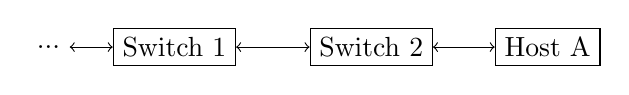
\begin{tikzpicture}
    \node[draw] (node1) at (-0.2,2.5) {Switch 1};
    \node[draw] (node2) at (2.3,2.5) {Switch 2};
    \draw[<->] (node1.east) -- (node2.west);
    \node[draw] (node3) at (4.54,2.5) {Host A};
    \draw[<->] (node2.east) -- (node3.west);
    \node (node4) at (-1.8,2.5) {...};
    \draw[<->] (node4.east) -- (node1.west);
  \end{tikzpicture}
  \caption{Topology of simple example network}
  \Description{Switch 1 is connected to Switch 2, which is connected to Host A. Switch is is also connected to the rest of the network via port 1.}
\end{figure}

Suppose we want to block all traffic originating outside of the local
subnet \texttt{10.0.0.0/24} from reaching Host A. Figure \ref{sample_program}
gives a Typed NetKAT program that models this behavior.

\begin{figure}
\begin{verbatim}
packet Ethernet {
  sw: int
  port: int
  src_mac: bits[48]
  dst_mac: bits[48]
  ethtype: bits[16]
  data:    any
}
packet IPv4 {
  src_ip: ip4_addr
  dst_ip: ip4_addr
}

let firewall: IPv4 = 
  if dst_ip = 10.0.0.1 then
    src_ip ~ 10.0.0.0/24
  else 1 in
let inbound_policy: Ethernet =
  if ethtype = 0x0800 then data as IPv4 {firewall} else 1 in
let forward: Ethernet = 
  (sw = 1; port = 1; sw := 2; port := 1)
  + (sw = 2; port = 2; sw := 1, port := 2)
  + (sw = 1; port = 2) + (sw = 2; port = 1) in
(inbound_policy; forward)*
\end{verbatim}

\caption{Example program written in Typed NetKAT}
\Description{An example NetKAT program that only allows requests to 10.0.0.1 if it originates from subnet 10.0.0.0/24.}
\label{sample_program}
\end{figure}

The \texttt{firewall} policy expects a packet of type \texttt{IPv4},
and it compares the destination IP address to 10.0.0.1. If the
destination IP is 10.0.0.1, it only accepts the packet if the
source IP matches the network prefix 10.0.0.0/24. If the 
destination IP is not 10.0.0.1, then the policy allows the packet.

\texttt{inbound\_policy} is run at each network hop. It checks if
the encapsulated data is an IPv4 packet by comparing the \texttt{ethtype}
field to 0x0800, the IEEE standard for IPv4. If the encapsulated
data is IPv4, then it runs the firewall policy. Otherwise, the packet
is accepted.

The \texttt{forward} policy represents the underlying network topology.
A packet that arrives on switch 1 port 1 is forwarded to switch 2's port 1.
A packet that arrives on switch 2 port 1 is accepted (we don't model the host,
so we just model this as the packet is accepted). A packet that arrives on
switch 2 port 2 originates from the host and is forwarded to switch 1 port 2.
A packet that arrives on switch 1 port 2 is forwarded left to the rest of the
network.

The final line of the program repeatedly runs our policy and forwards the
packet if it is accepted, using the Kleene star operator. We assume all
packets on the network are Ethernet packets. Note that \texttt{sw} and
\texttt{port} are not actual Ethernet fields. Instead, these are special
fields used to indicate a packet's location in the physical network.

\subsection{New Syntax, Type Rules, and Semantics}

We extend \citet{anderson2014netkat}'s NetKAT with the new syntax for
policies

\[
  p ::= \cdots\ |\ f_i \textsf{ as T }  \{ p \}
\]

This new syntax is used to cast a field to a given type and run a policy
on the value of the field. In the example program, we ran the 
\texttt{firewall} policy on the \texttt{data} field of the Ethernet
casted to an IPv4 packet. All other syntax remains the same as
Anderson's original NetKAT.

We also define typing rules for NetKAT syntax. 
\[ \tau ::= \mathtt{int}_n\ |\ \mathtt{uint}_n\ |\ \mathtt{bits}_n\ |\ \mathtt{ip4\_addr}\ |\ N\ |\ N \to N\ |\ \mathtt{any} \]
where $N$ is a named packet type.

Let $\Gamma$ be a type context and $\Sigma$ be the name context.

\[
  \Gamma ::= \cdot\ |\ \Gamma, f: \tau \qquad \Sigma := N \mapsto \{f_1: \tau_1, \dots, f_k: \tau_k\}
\]

\[
  \infer{\Gamma \vdash f_i \textsf{ as T } \{ p \}: \tau \to \tau}{\Gamma \vdash f_i: \tau_i & \Sigma(T) \vdash p: \mathsf{T} \to \mathsf{T} & \mathsf{T} <: \tau_i}
\]

For brevity, we will not include all type rules. But note that for all policies,
the output type is the same as the input type because no syntax changes the
type of the packet.

Finally, we define semantics for this new syntax.

\[ \llbracket f \textsf{ as T } \{ p \} \rrbracket\ (pk::h) = \bigcup_{h' \in \llbracket p \rrbracket(pk.f::\langle\rangle) } \{ [pk[f := x]\ |\ x \in h'] \concat h \} \]

$\concat$ is the concatenation operator defined recursively as
\[ (x::xs) \concat ys = x :: (xs \concat ys) \qquad \langle\rangle \concat ys = ys. \]

When we perform the focus policy, we first evaluate policy $p$ on the 
value of the specified field. For each subhistory this evaluation yields, 
we set field's value to the subpacket for each subpacket in the 
subhistory, and we concatenate list with the rest of the packet's history.

%What you have accomplished since the proposal: tasks completed, results
%so far, and any new related work you have identified, e.g.
%\citet{pierce2002}.

\section{Planned Changes}
The goal of compiling to the original untyped NetKAT was more difficult
to implement than we anticipated. This any type can be in the \texttt{any}
packet type, so fixed field mappings will not work. For example, if we had
a tunneling protocol like VXLAN, then an Ethernet packet would contain
another Ethernet packet after a few layers of nesting. Even though these
two types are both Ethernet, they must have distinct field mappings.

We discussed a couple of ways to mitigate this. One was to drop the
goal of compiling to untyped NetKAT altogether, and instead write our
own verifier based on the semantics of NetKAT. Another approach was to
force every packet to be \texttt{Ethernet<T>} (e.g. \texttt{Ethernet<ARP>} or \texttt{Ethernet<IPv4<any>>}). Then if we had \\\texttt{Ethernet<IPv4<IPv4<any>>>}, we create manual mappings by offsetting
the nested types with the sum of the sizes of the outer types.

We decided to implicitly track each type as \texttt{T<offset>}. These
offsets are invisible to the programmer, but the compiler will
automatically infer these offsets based on the size of previous
types. Take our \texttt{Ethernet} that contains an \texttt{IPv4},
for example. Our type would actually look like

\begin{verbatim}
packet Ethernet<offset> {
  src_mac: bits[48]
  dst_mac: bits[48]
  ethtype: bits[16]
  data:    any<offset+112>
}
\end{verbatim}

When we cast \texttt{any} to \texttt{IPv4} with 
\texttt{data as IPv4 \{...\}}, the compiler implicitly treats it as a cast 
to \texttt{IPv4<112>}. It then compiles all the bitmappings for 
\texttt{IPv4} offset by 112 bits.

One caveat of this approach is that each packet type must have at most one
field with \texttt{any} type.

Other approaches we considered were using dependent types. This maps
cleanly to our use case for modeling networks because in many network
protocols, the value of one field is used to determine how to interpet
another field. For example, the \texttt{ethtype} field in Ethernet
determines what protocol is encapsulated. But to limit the scope of this
project, we decided to leave properly checking these values as the
responsibility of the programmer.

% Any issues you have found with your original proposal, and the changes
% to your research plan for the remaining time before the final report
% (December 10).

\bibliographystyle{ACM-Reference-Format}
\bibliography{references}

\end{document}
